\begin{frame}{Quantifying  Separation}
	\textbf{Possible Track Separation Variables}
	\begin{itemize}
		\item $\Delta R_{0, 1}$ : Separation between the electron and positron at the first/last tracking station in the x-y plane
		\item $\theta_{0, 1}$ : Angle between the line connection decay vertex to the two tracks at the first/last tracking station
		% \item $\Phi_{p0}$ [To be Removed]
		\item $\Delta X_{0,1}$ : Same as above but only in x direction 
		\item $\Delta Y_{0,1}$ : Same as above but only in y direction
		\item $\Delta R_P = \sqrt{\Delta \eta ^2 + \Delta \phi^2}$  : Momentum space separation between electron and positron
	\end{itemize}

	\textbf{\footnotesize Notes:}
	\begin{itemize}
		\scriptsize
		\item Particle predominantly separated in the y-direction due to magnetic field
		\item DeltaX looks symmetric but separation here is much lower.[DeltaR $\approx$ DeltaY]
		\item DeltaRP[=ROOT::Math::VectorUtil::DeltaR(d0\_momenta, d1\_momenta)] has a relatively ``flat'' distribution and is not a good separation metric
		\item We shall use DeltaR and Theta as the primary separation variables
	\end{itemize}
\end{frame}





\begin{frame}{Track Separation Calculations}
	\begin{figure}
		\begin{tikzpicture}[scale=1]
			% Define Mother and daughter particles
			\coordinate(M) at (-1, 0);
			\coordinate(d1) at (3, 1);
			\coordinate(d2) at (3, -1);
		
			% Draw grid
			\draw[step=1cm,gray!30,very thin] (-2, -2) grid (6, 2);
			\draw[-,thick] (3,-2) -- (3,2) node[pos=0.95, left] {Tracking Station 1};
			\draw[->, thick](3, 0) -- (3.5, 0) node[right] {$z$};
			
			% Draw mother and daughter particles
			\filldraw (M) circle (2pt) node[above] {A' (M)};
			\filldraw (d1) circle (2pt) node[above right] {positron (d0)};
			\filldraw (d2) circle (2pt) node[below right] {electron (d1)};
			\draw[->, thick, red] (d1) + (3,0) -- ($ (d2) + (3,0) $) node[midway, left] {DeltaR0};
	
			\draw[dashed] (M) -- (d1);
			\draw[dashed] (M) -- (d2);
		
		% Draw arc and label the angle
		\draw[<->, thick, red] (M)+({atan(1/4)}:1) arc ({atan(1/4)}:{atan(-1/4)}:1) node[midway, right] {Theta0};
		
		\end{tikzpicture}
		\caption{Angle and separation between the particles defined}	
	
	\end{figure}

	\textbf{Calculation of Separation Variables}
	\begin{itemize}
		\small
		\item Separation variables are calculated using MC-truth data.
		\item This ensures consistency across both ALMA9 and CENTOS7.
		\item The separation variables used are :
		\begin{itemize}
			\scriptsize
			\item truthd0\_x, truthd0\_y, truthd1\_x, truthd1\_y, truthd0\_z, truthd1\_z
			\item They are vectors containing the ``truth positions'' of d0 ($e+$) and d1 ($e-$): 
			\item at the vertex, the first, second, and third tracking stations.
		\end{itemize}
	\end{itemize}
	
\end{frame}


% \begin{frame}[fragile]{Code snips Test}
% 	\begin{minted}{python}
% 		#include <iostream>
% 		int main() {
% 			std::cout << "Hello, World!";
% 			return 0;
% 		}
		
% 	\end{minted}
% \end{frame}

% \begin{frame}[fragile]{Code Snippet for Separation Calculation}
% 	\centering
% 	\begin{figure}
% 		\hspace{-1cm}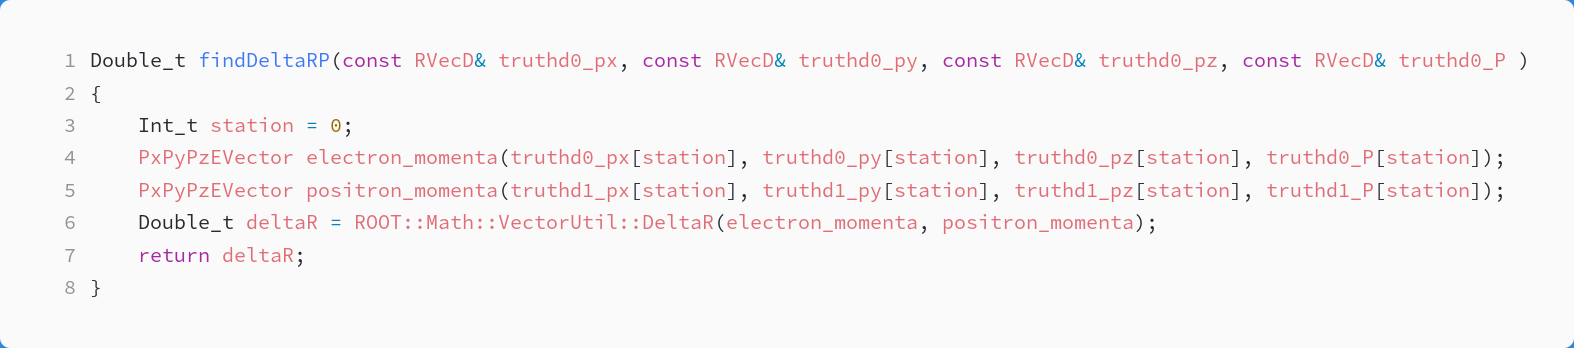
\includegraphics[width=\linewidth]{./assets/code_snip1.png}
% 	\end{figure}
% 	\begin{figure}
% 		\hspace{-1cm}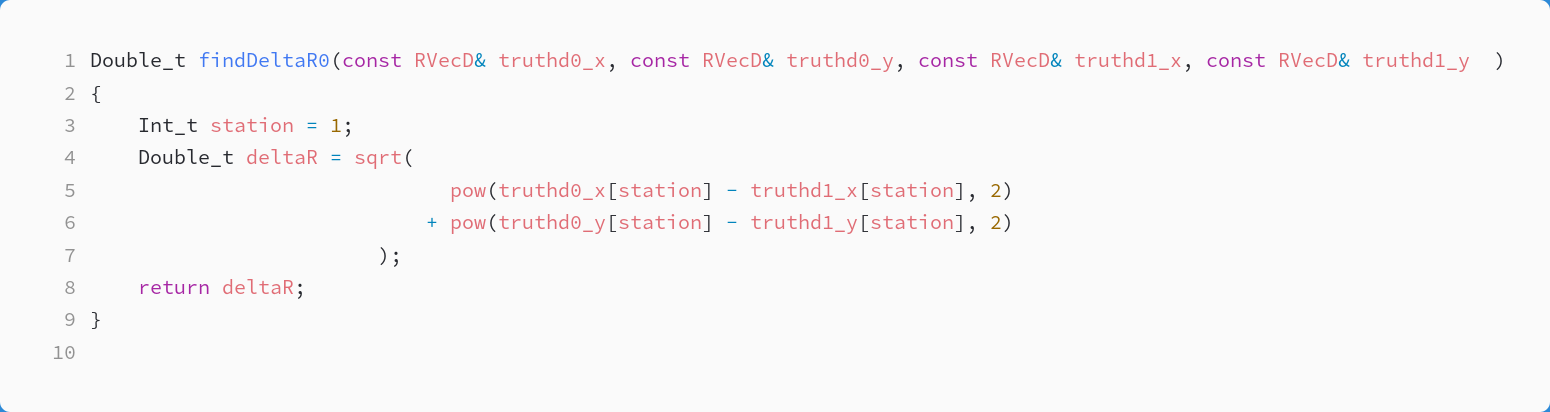
\includegraphics[width=\linewidth]{./assets/code_snip2.png}
% 	\end{figure}
% 	\begin{figure}
% 		\hspace{-1cm}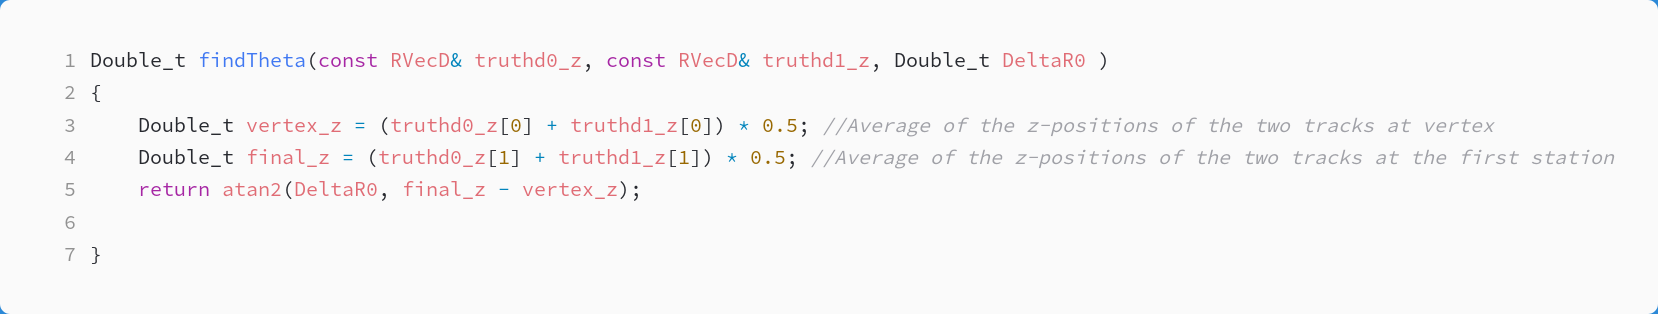
\includegraphics[width=\linewidth]{./assets/code_snip3.png}
% 	\end{figure}
% \end{frame}

% \begin{frame}{Calculation of the Separation Variables}
% \end{frame}

% \begin{frame}{Distribution of DeltaR1}
% 	\begin{figure}
% 		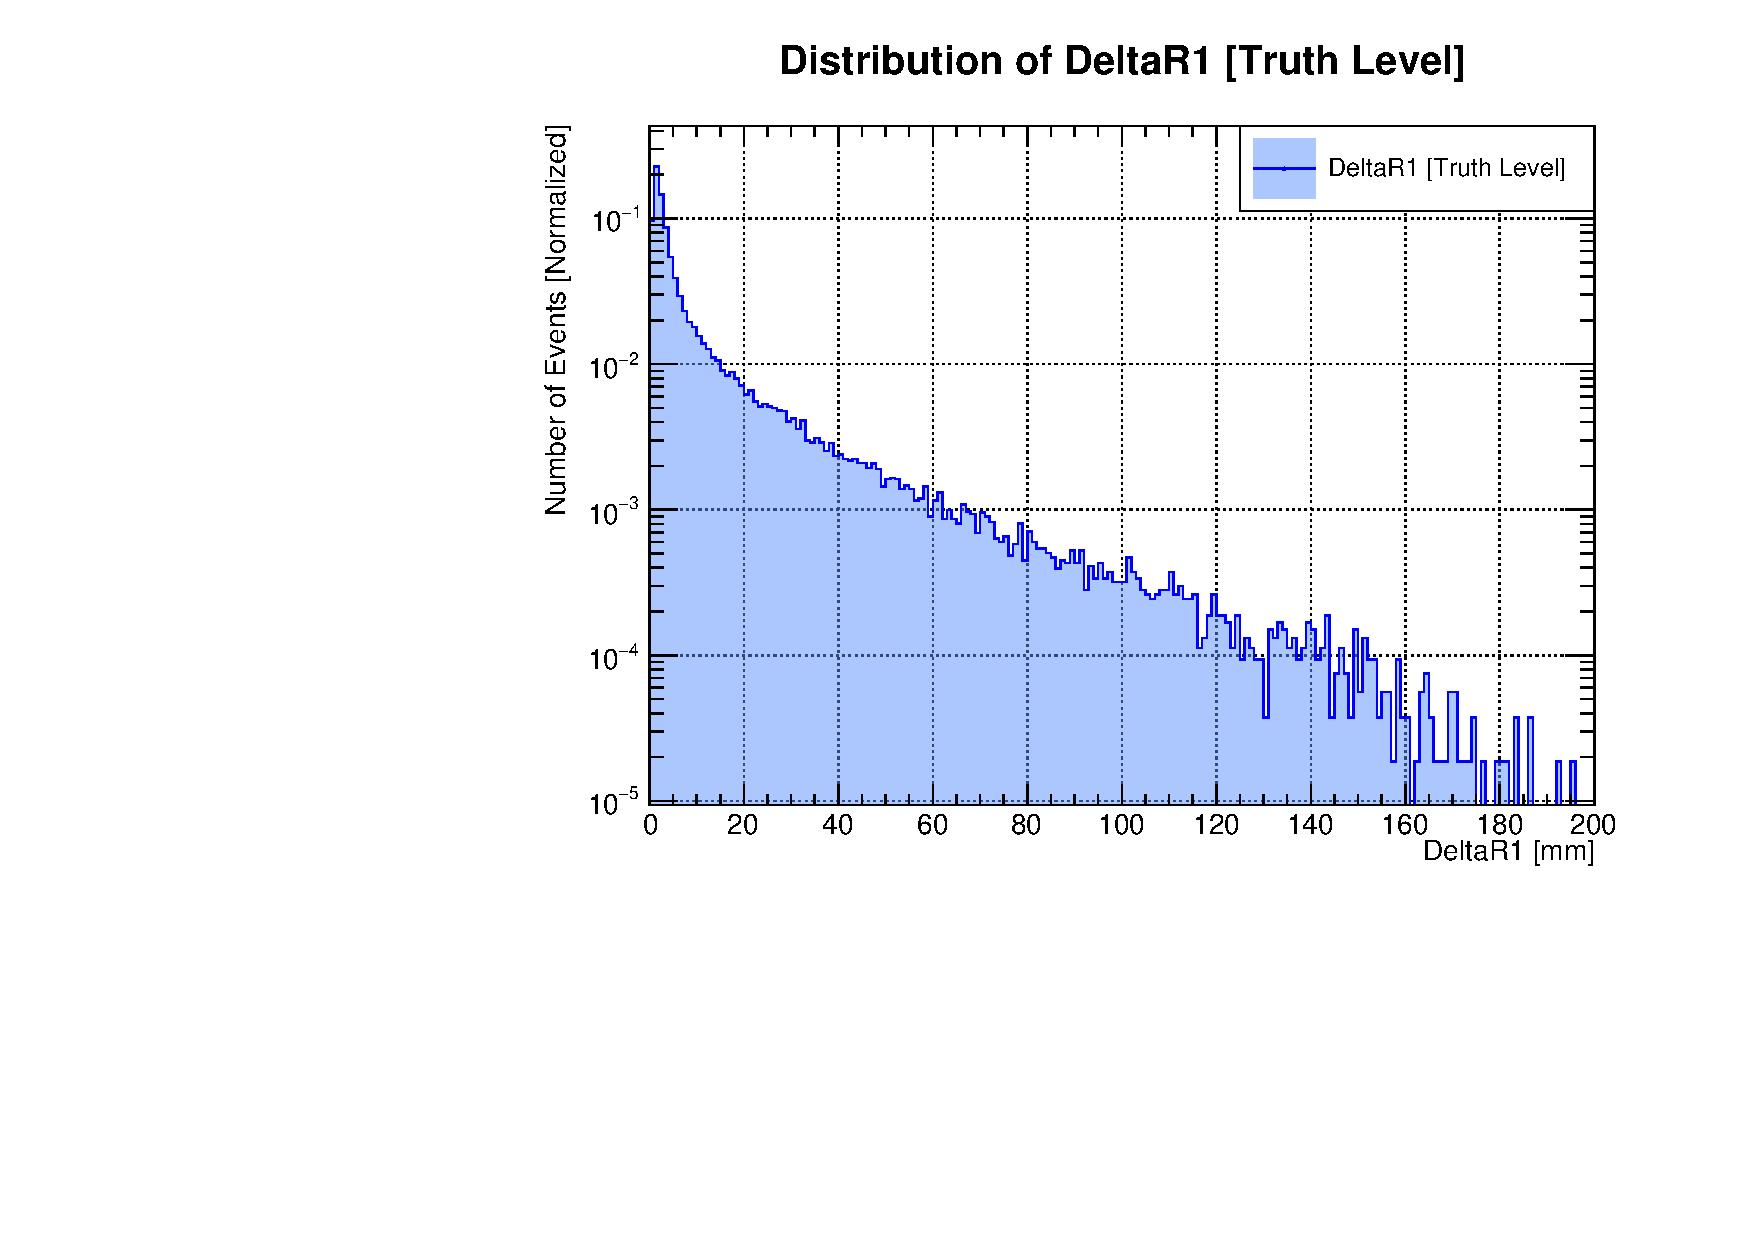
\includegraphics[width=\linewidth]{./output/DeltaR1.pdf}
% 	\end{figure}
% \end{frame}

% \begin{frame}{Distribution of DeltaR0}
% 	\begin{figure}
% 		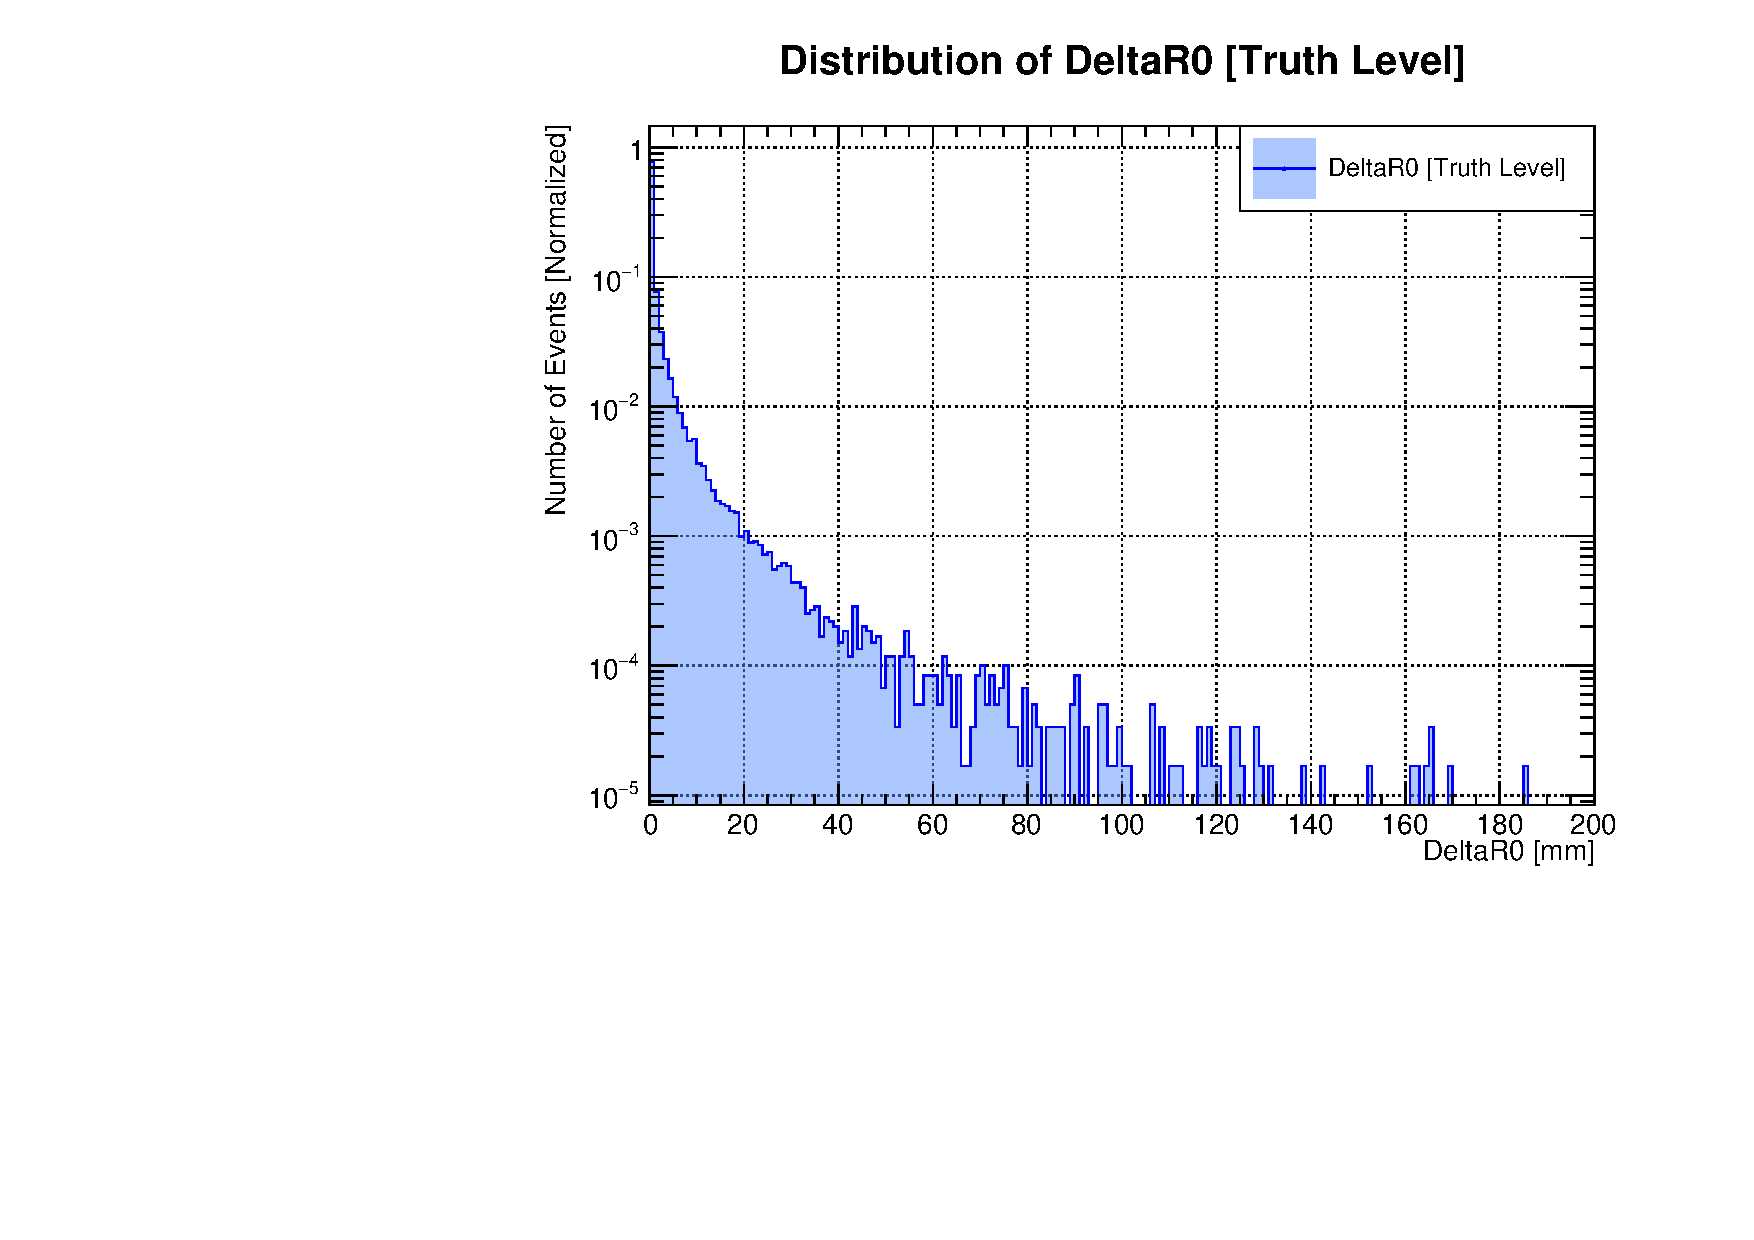
\includegraphics[width=\linewidth]{./output/DeltaR0.pdf}
% 	\end{figure}
% \end{frame}

\begin{frame}{Distribution of DeltaR}
	\begin{columns}
		\begin{column}{0.5\linewidth}
			\begin{figure}
				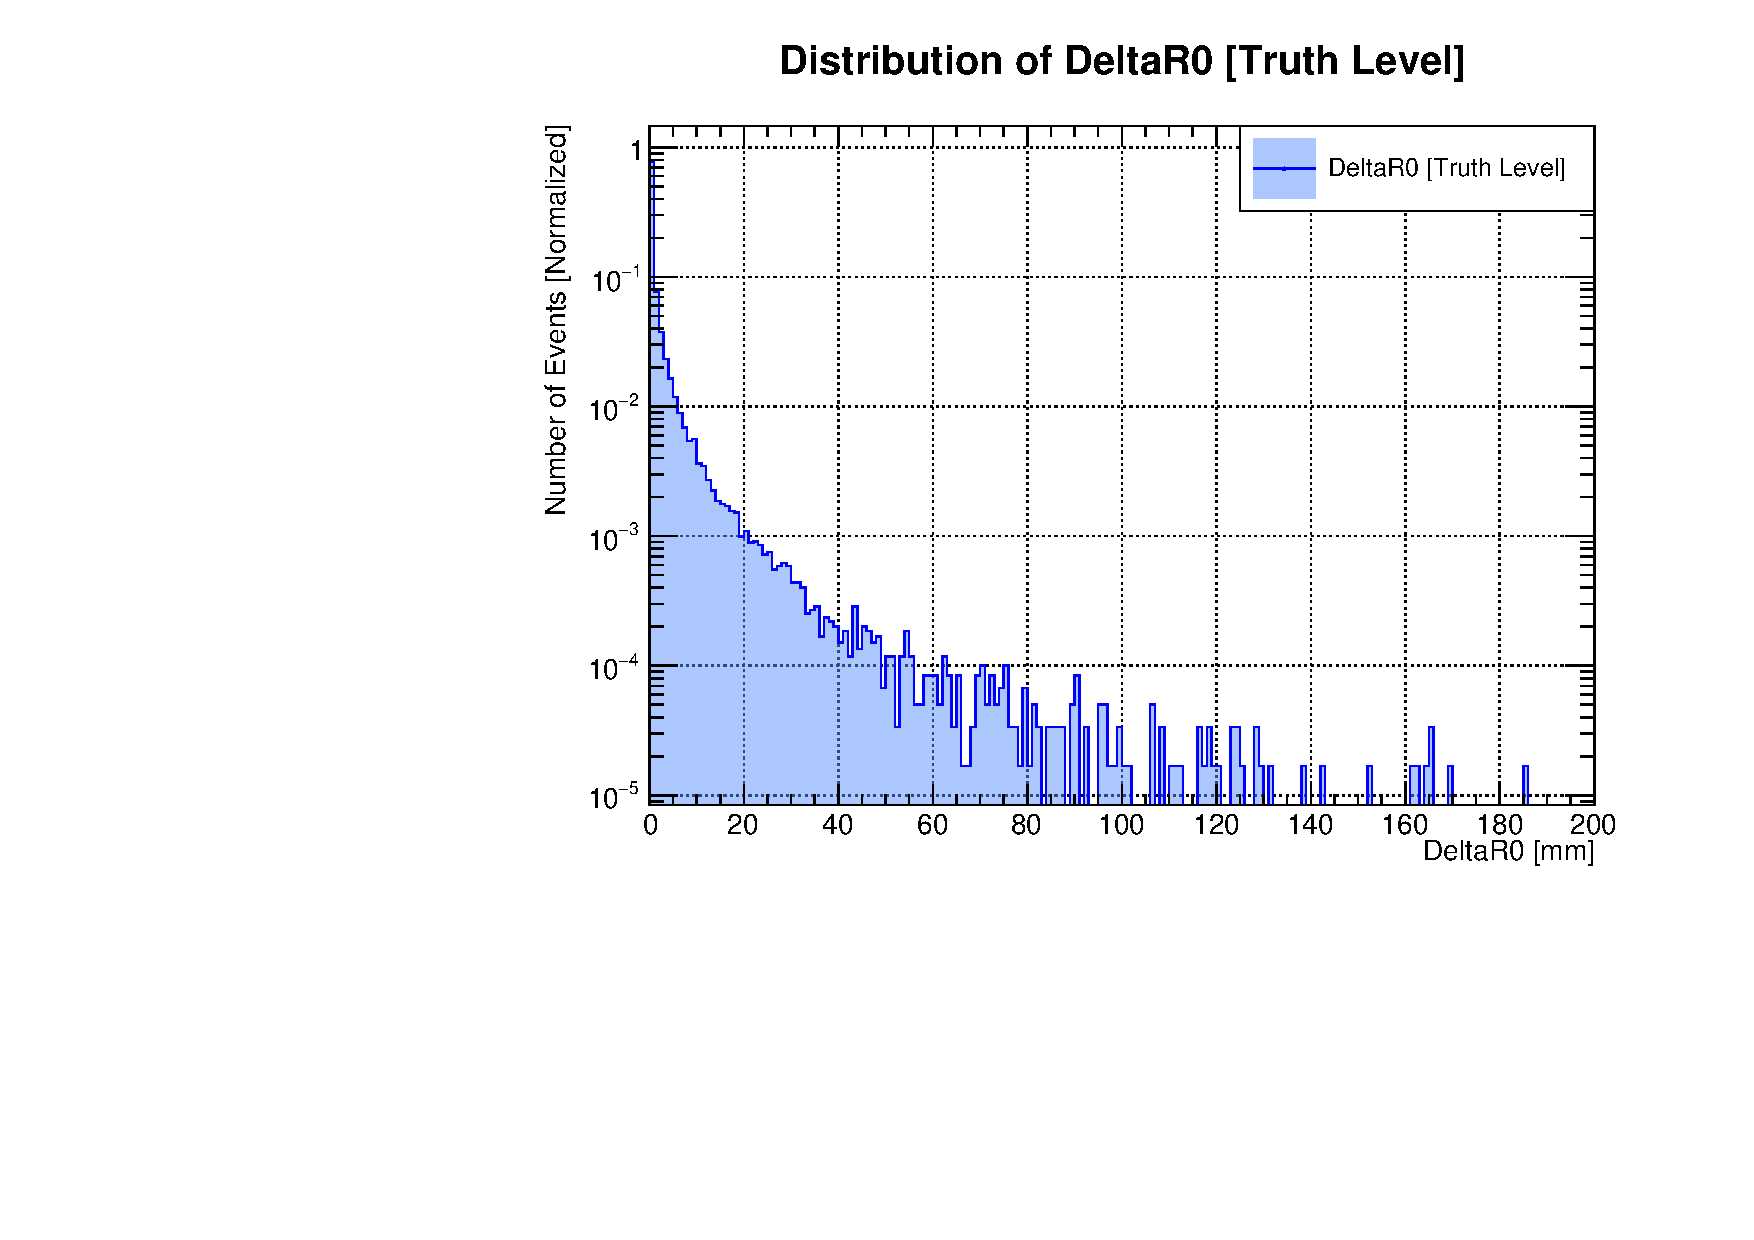
\includegraphics[width=\linewidth]{./output/DeltaR0.pdf}
				\caption{\tiny Distribution of DeltaR0 [DeltaR at Station 1]}
			\end{figure}
		\end{column}
		\begin{column}{0.5\linewidth}
			\begin{figure}
				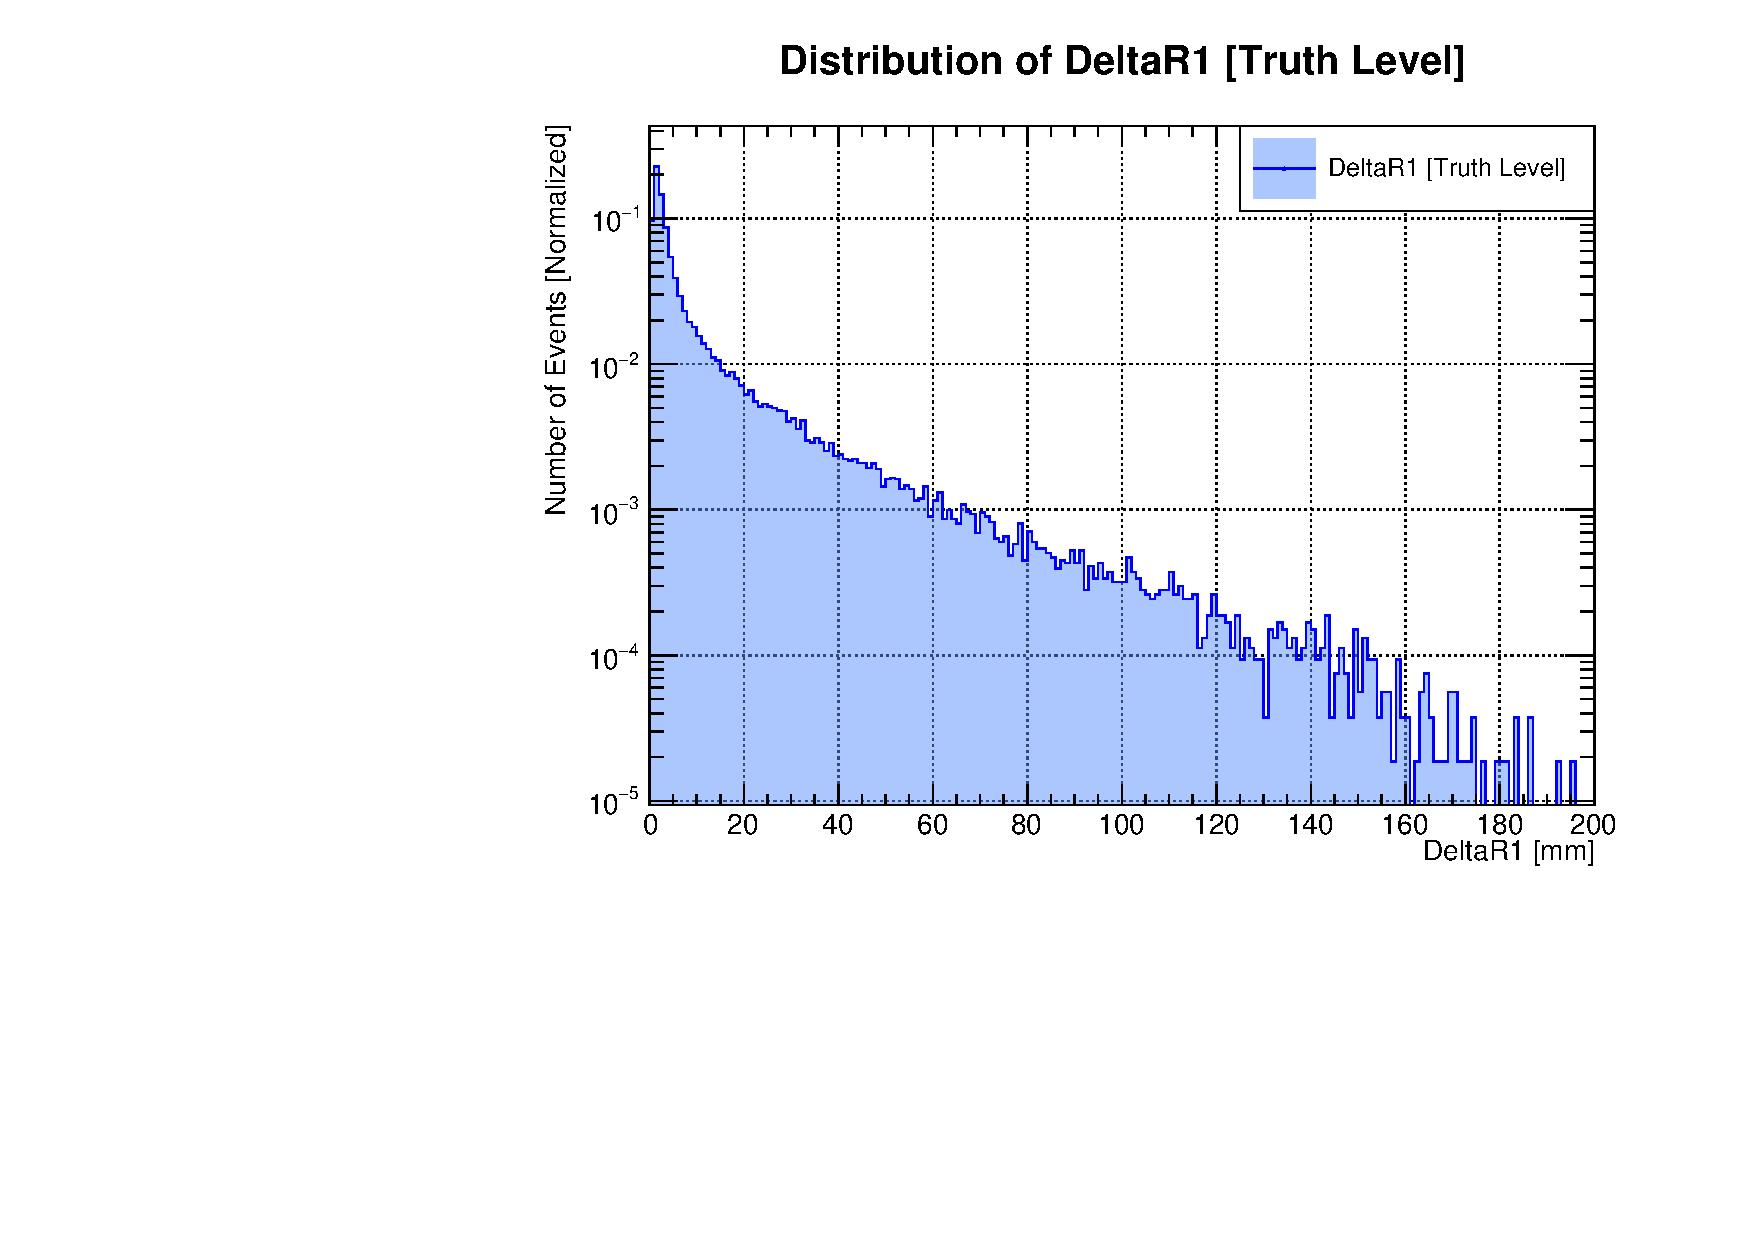
\includegraphics[width=\linewidth]{./output/DeltaR1.pdf}
				\caption{\tiny Distribution of DeltaR1 [DeltaR at Station 3]}
			\end{figure}
		\end{column}
	\end{columns}
	\vspace{0.5cm}
	\begin{itemize}
		\scriptsize
		\item NEvents decreases with increasing separation as expected
		\item Separations increase at the last tracking station due to the magnetic field
		\item Large separations at Station1 [$>$30 mm] aren't reconstructed at Station3
	\end{itemize}
\end{frame}

\begin{frame}{Transfer Plot between DeltaR0 and DeltaR1}
	\begin{figure}
		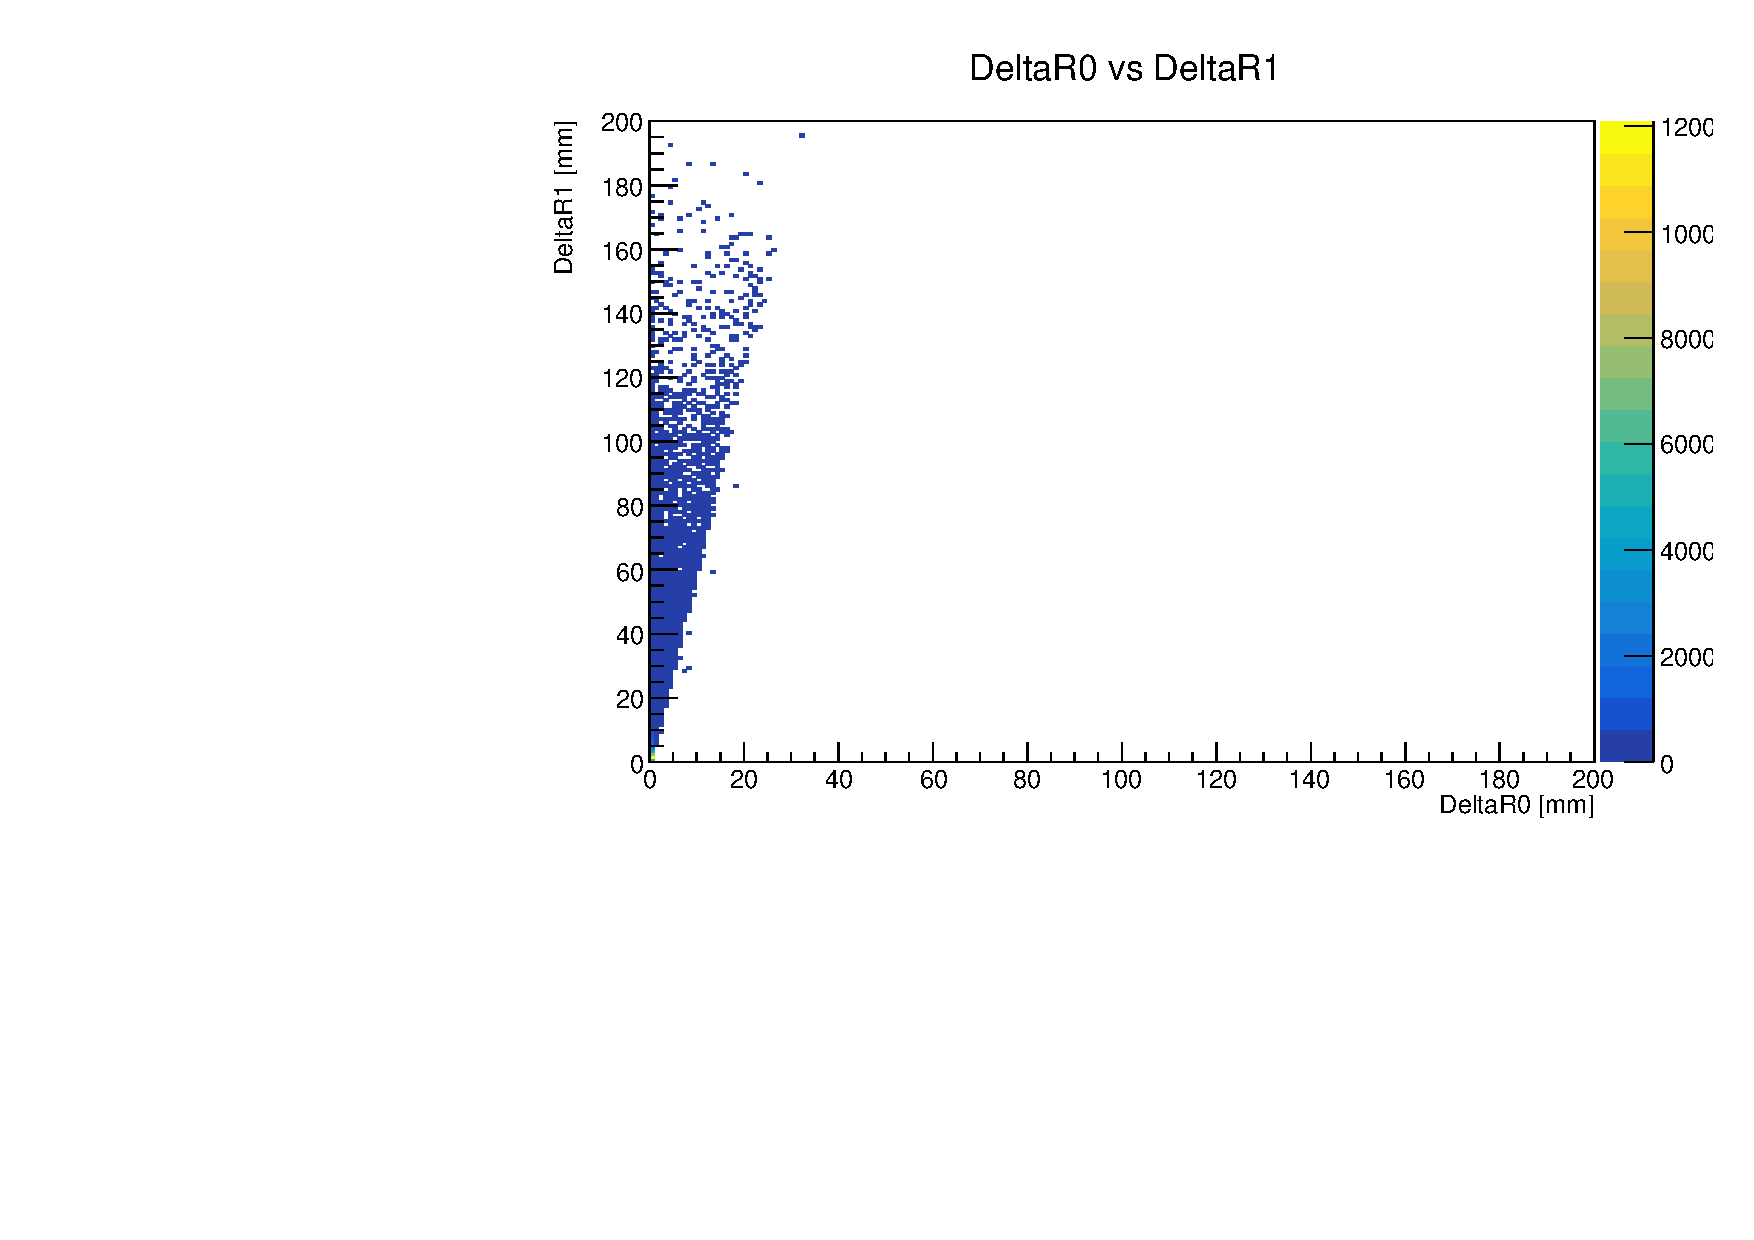
\includegraphics[width=\linewidth]{output/DeltaR0 vs DeltaR1.pdf}
	\end{figure}
\end{frame}

% \begin{frame}{Distribution of Theta0}
% 	\begin{figure}
% 		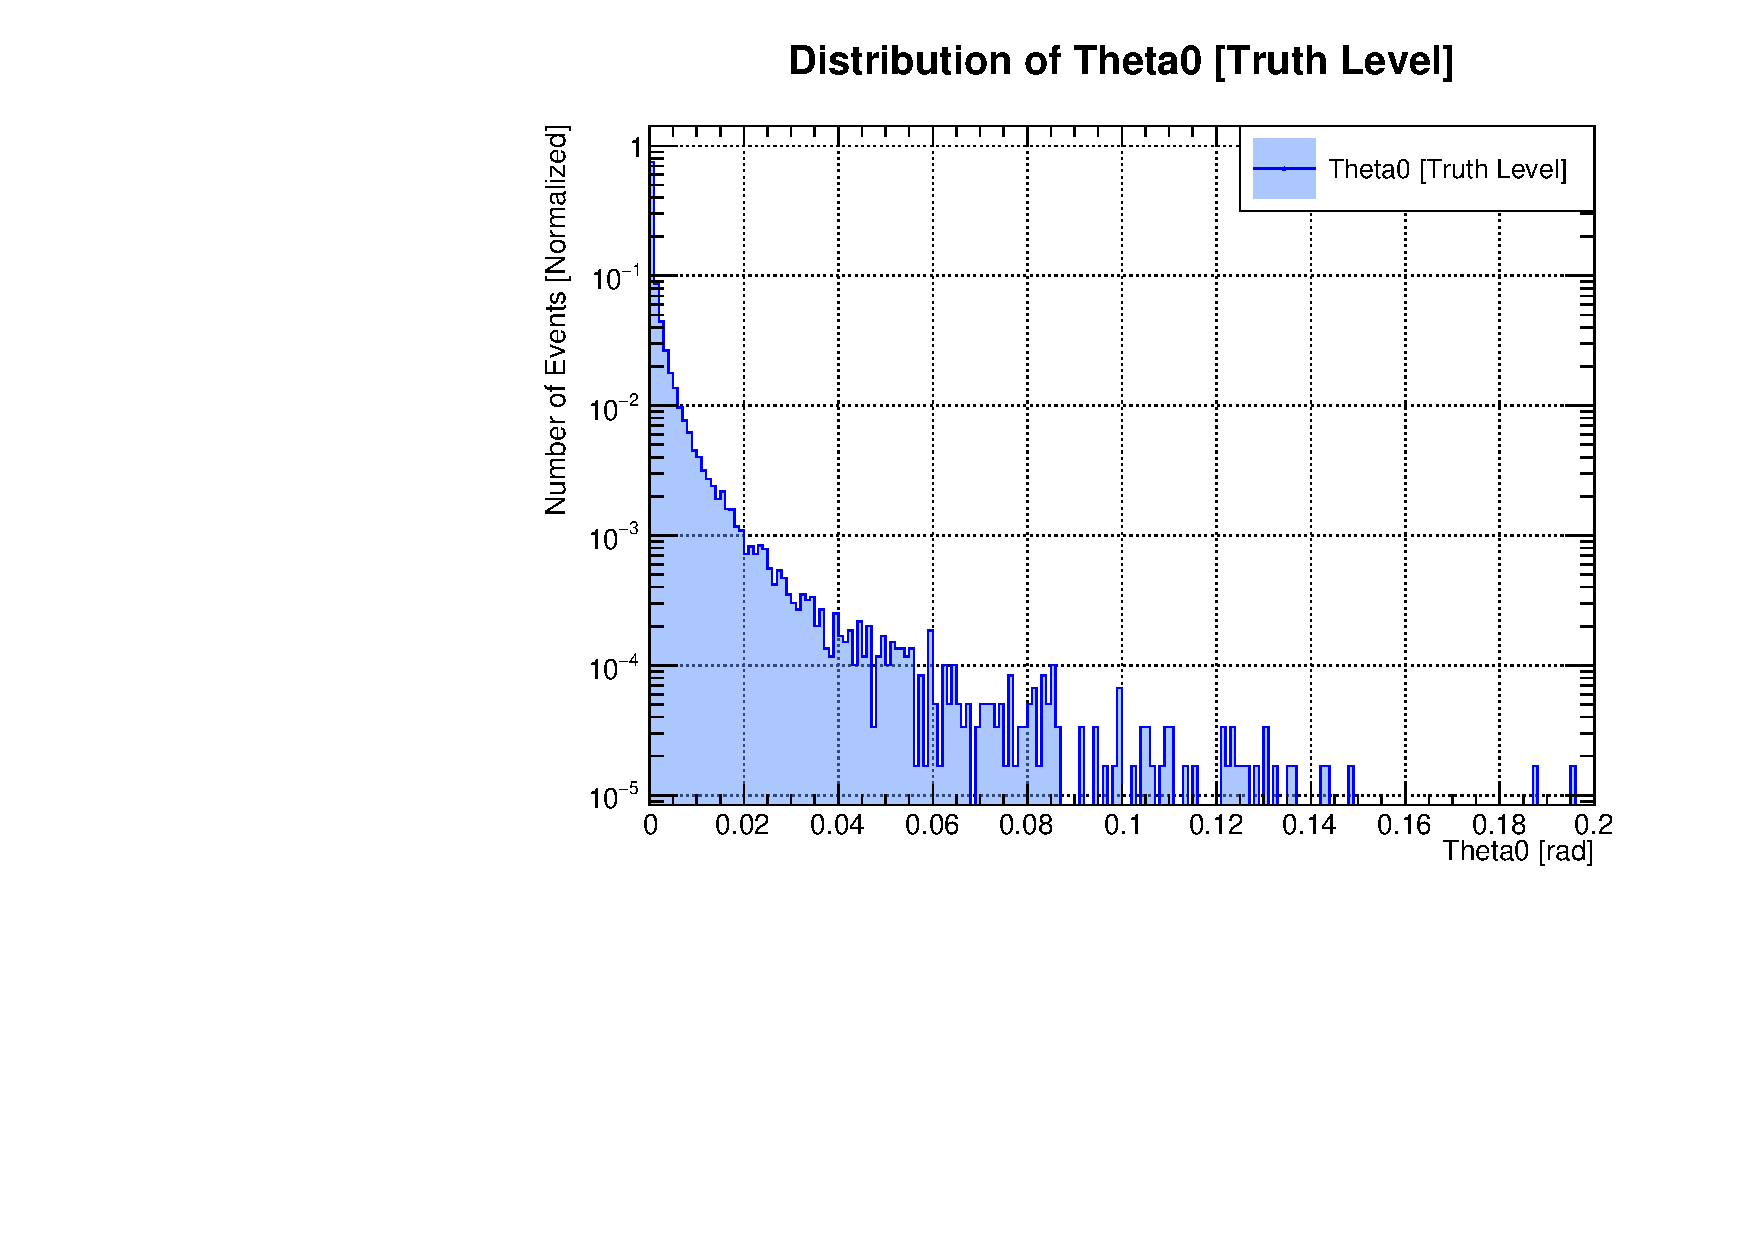
\includegraphics[width=\linewidth]{output/Theta0.pdf}
% 	\end{figure}
% \end{frame}
% \begin{frame}{Distribution of Theta1}
% 	\begin{figure}
% 		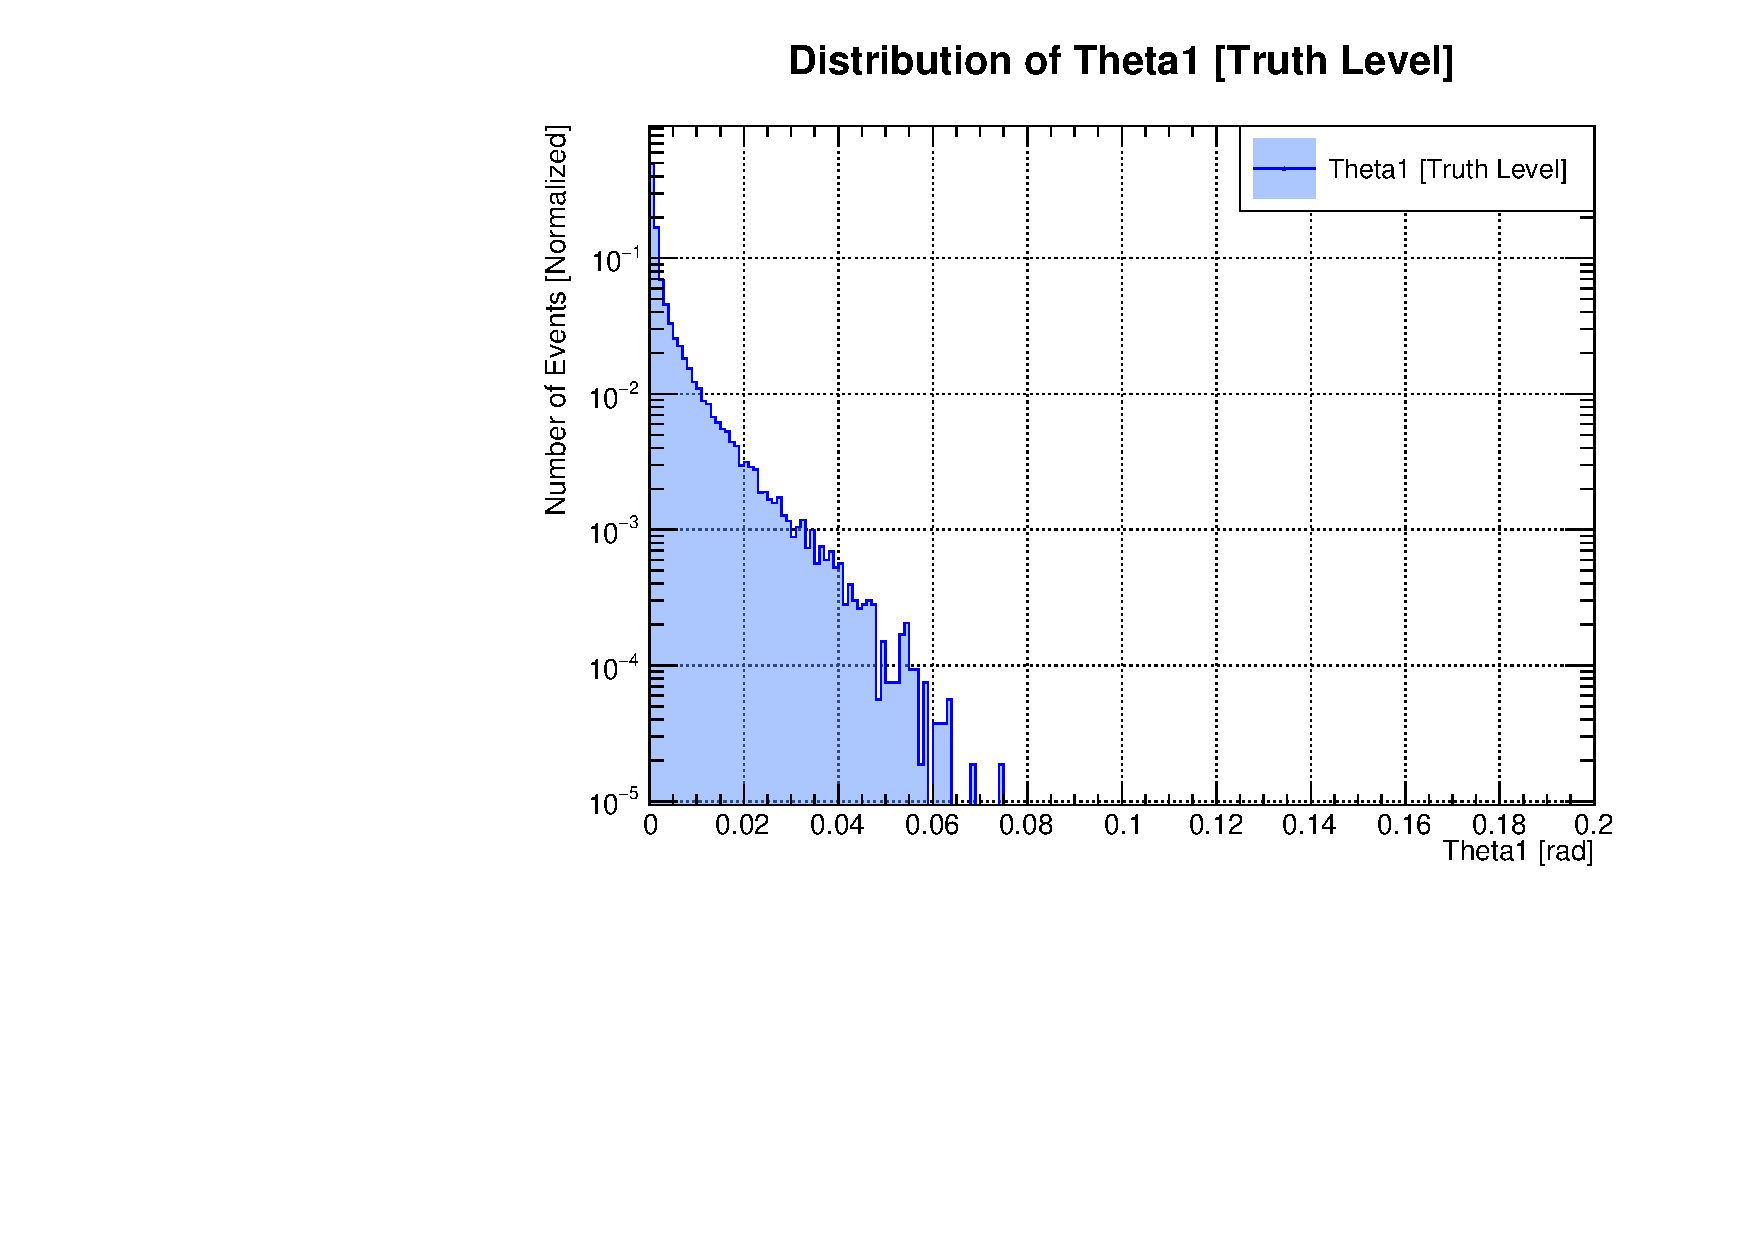
\includegraphics[width=\linewidth]{output/Theta1.pdf}
% 	\end{figure}
% \end{frame}

\begin{frame}{Distribution of Theta}
	\begin{columns}
		\begin{column}{0.5\linewidth}
			\begin{figure}
				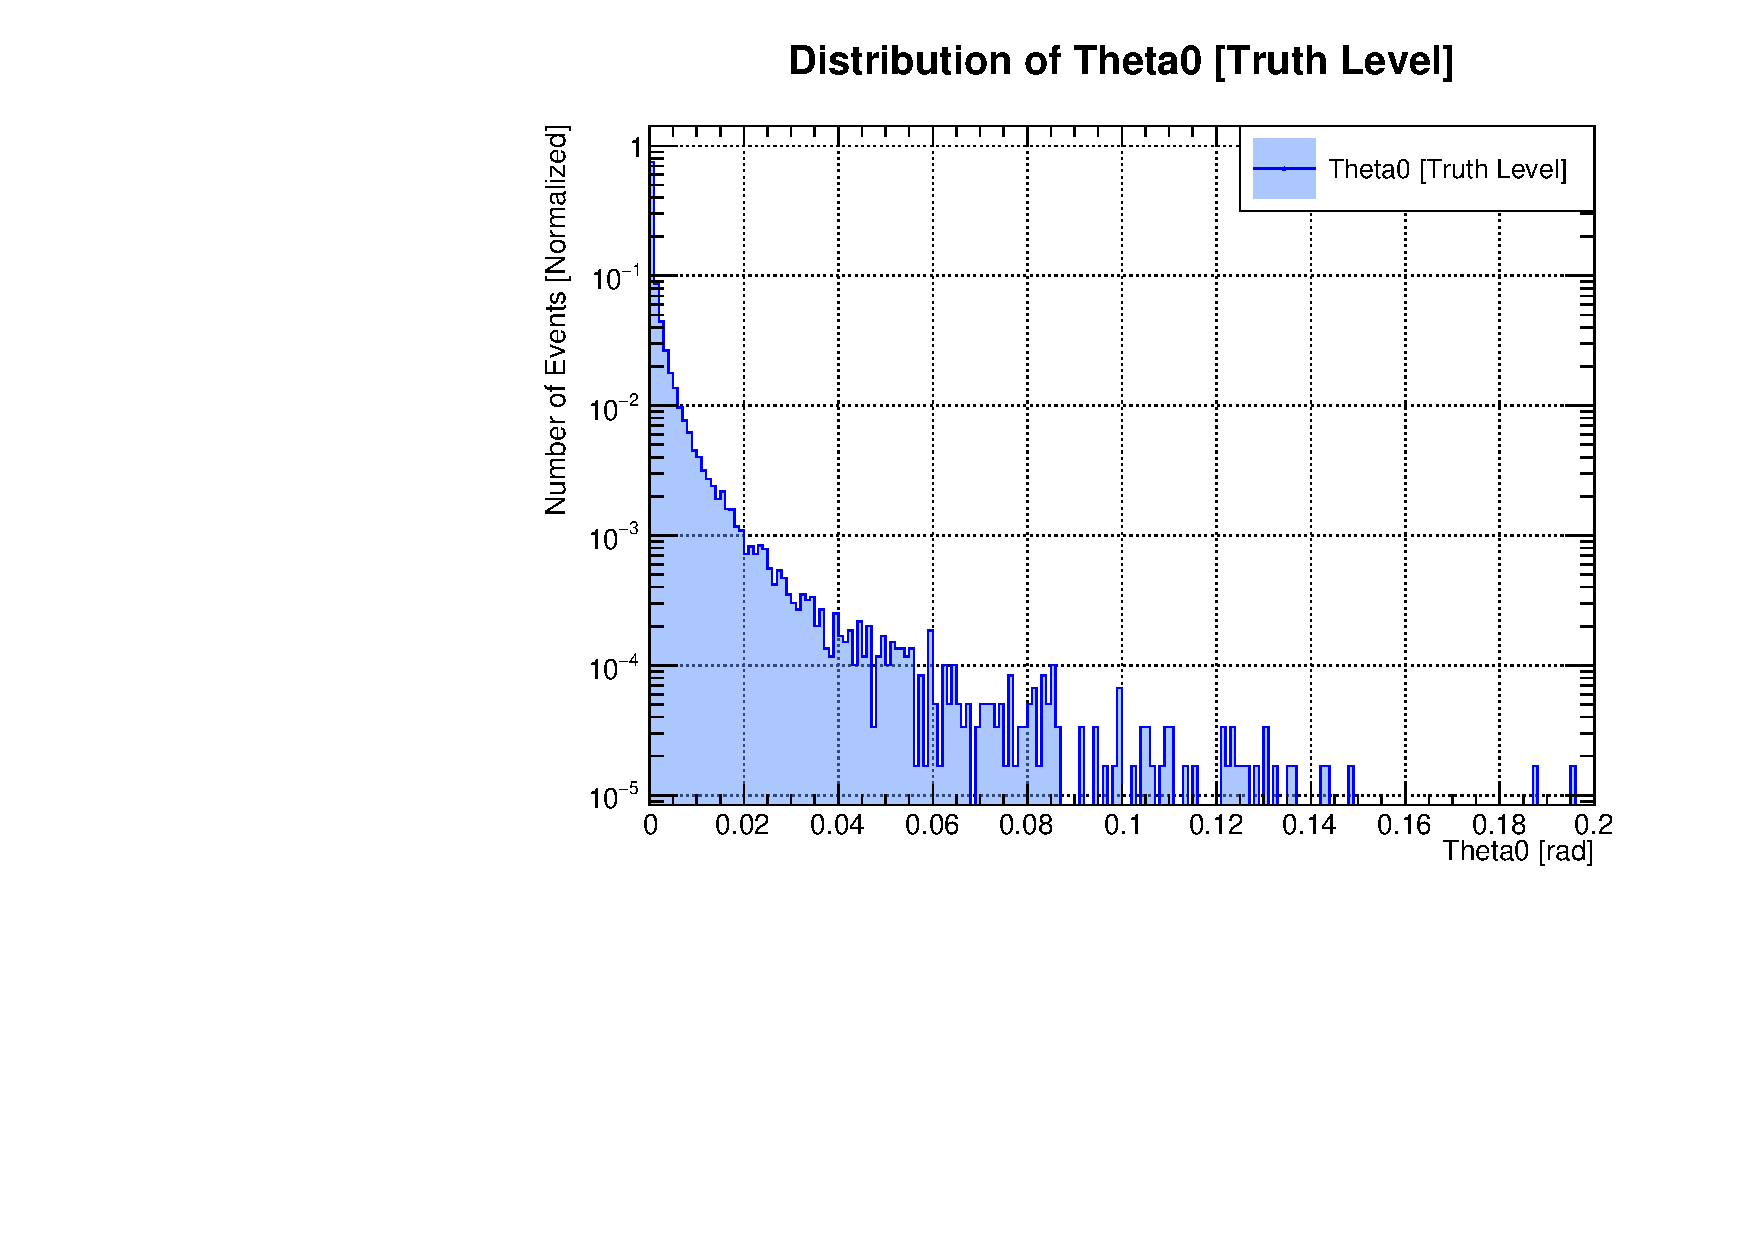
\includegraphics[width=\linewidth]{./output/Theta0.pdf}
				\caption{\tiny Distribution of Theta0 [Theta at Station 1]}
			\end{figure}
		\end{column}
		\begin{column}{0.5\linewidth}
			\begin{figure}
				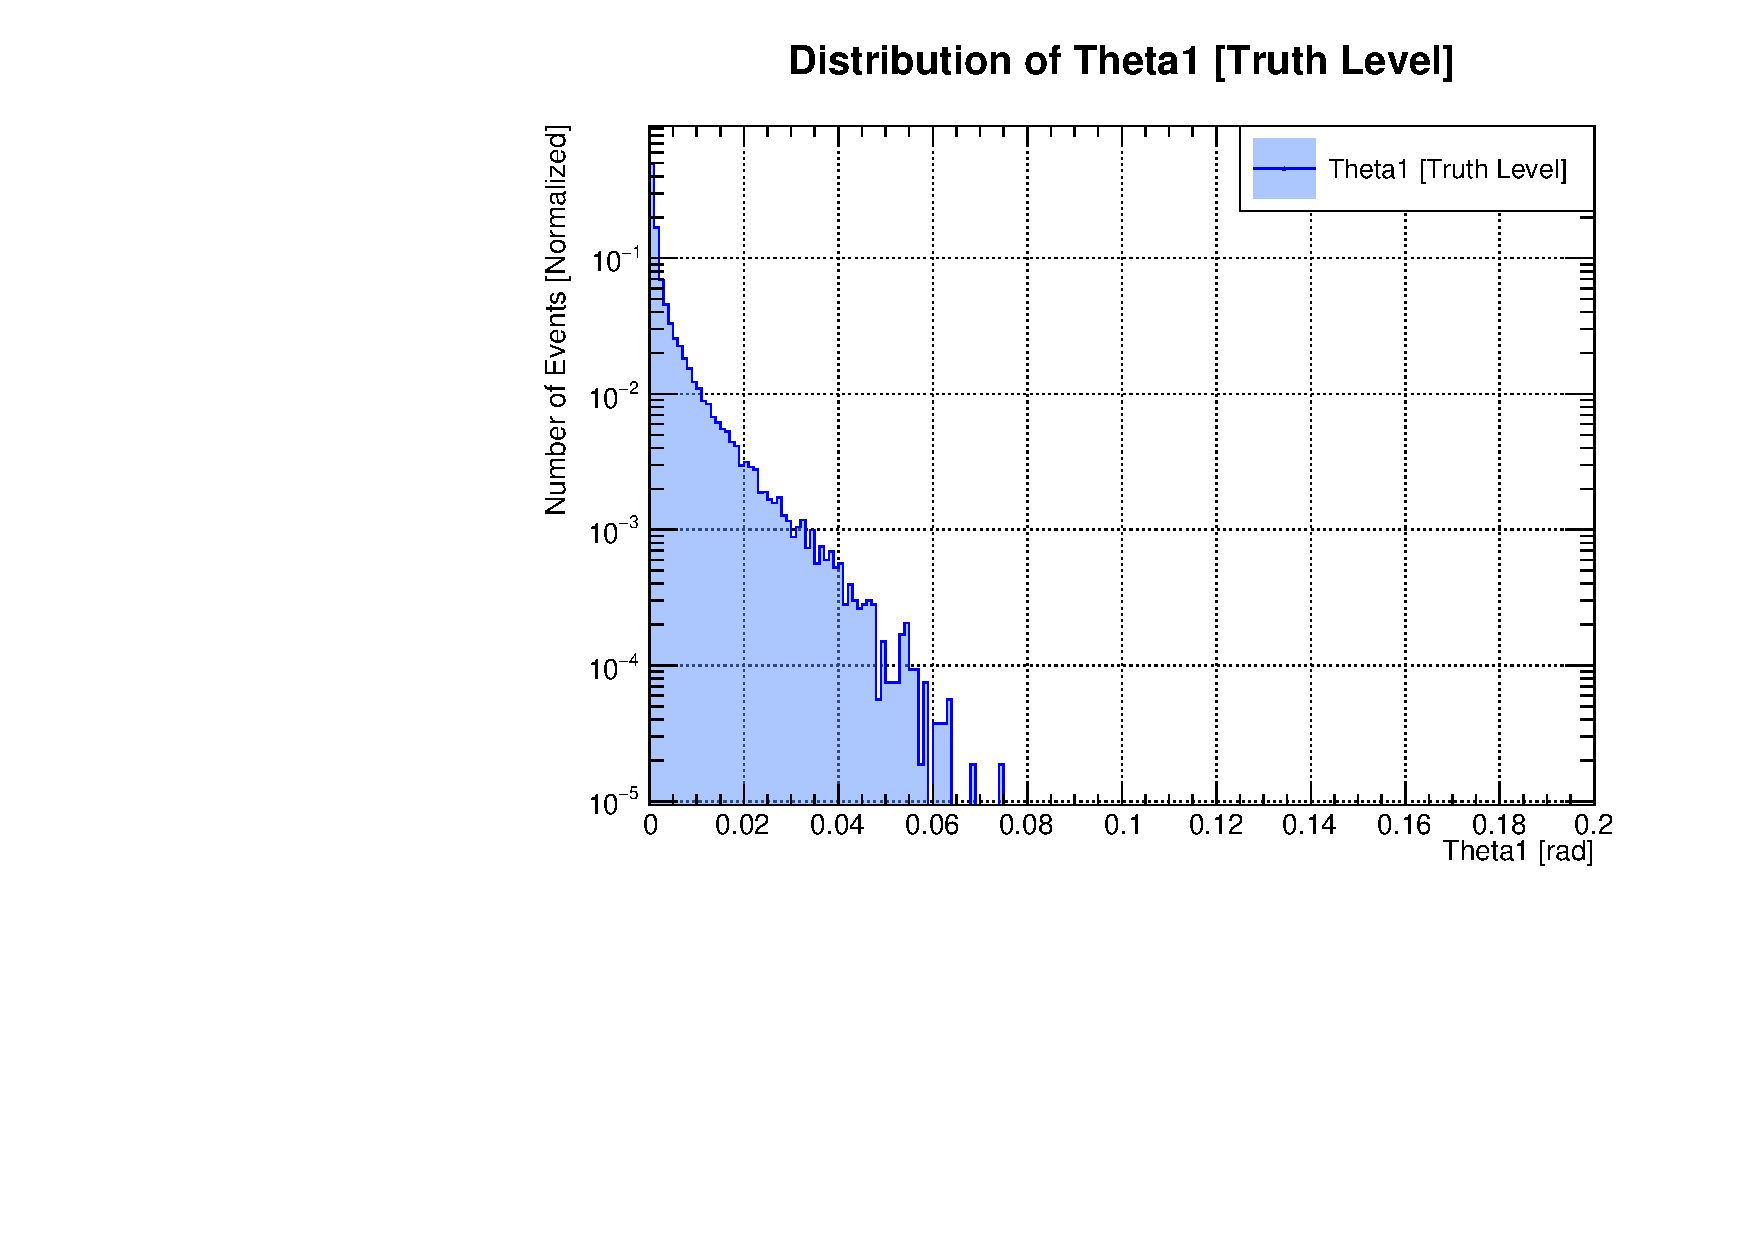
\includegraphics[width=\linewidth]{./output/Theta1.pdf}
				\caption{\tiny Distribution of Theta1 [Theta at Station 3]}
			\end{figure}
		\end{column}
	\end{columns}
	\vspace{0.5cm}
	\begin{itemize}
		\scriptsize
		\item As previously seen, separations increases at the last tracking station.
		\item Large separations at Station1 [$>$0.03 rad] aren't reconstructed at Station3
		\item Minimum angle for which a track can still go through the tracking spectrometer 0.083 rad [$\arctan{\frac{0.2 m}{2.4 m}}$, without accounting for the magnetic field]
	\end{itemize}
\end{frame}

\begin{frame}{Transfer Plot between Theta0 and Theta1}
	\begin{figure}
		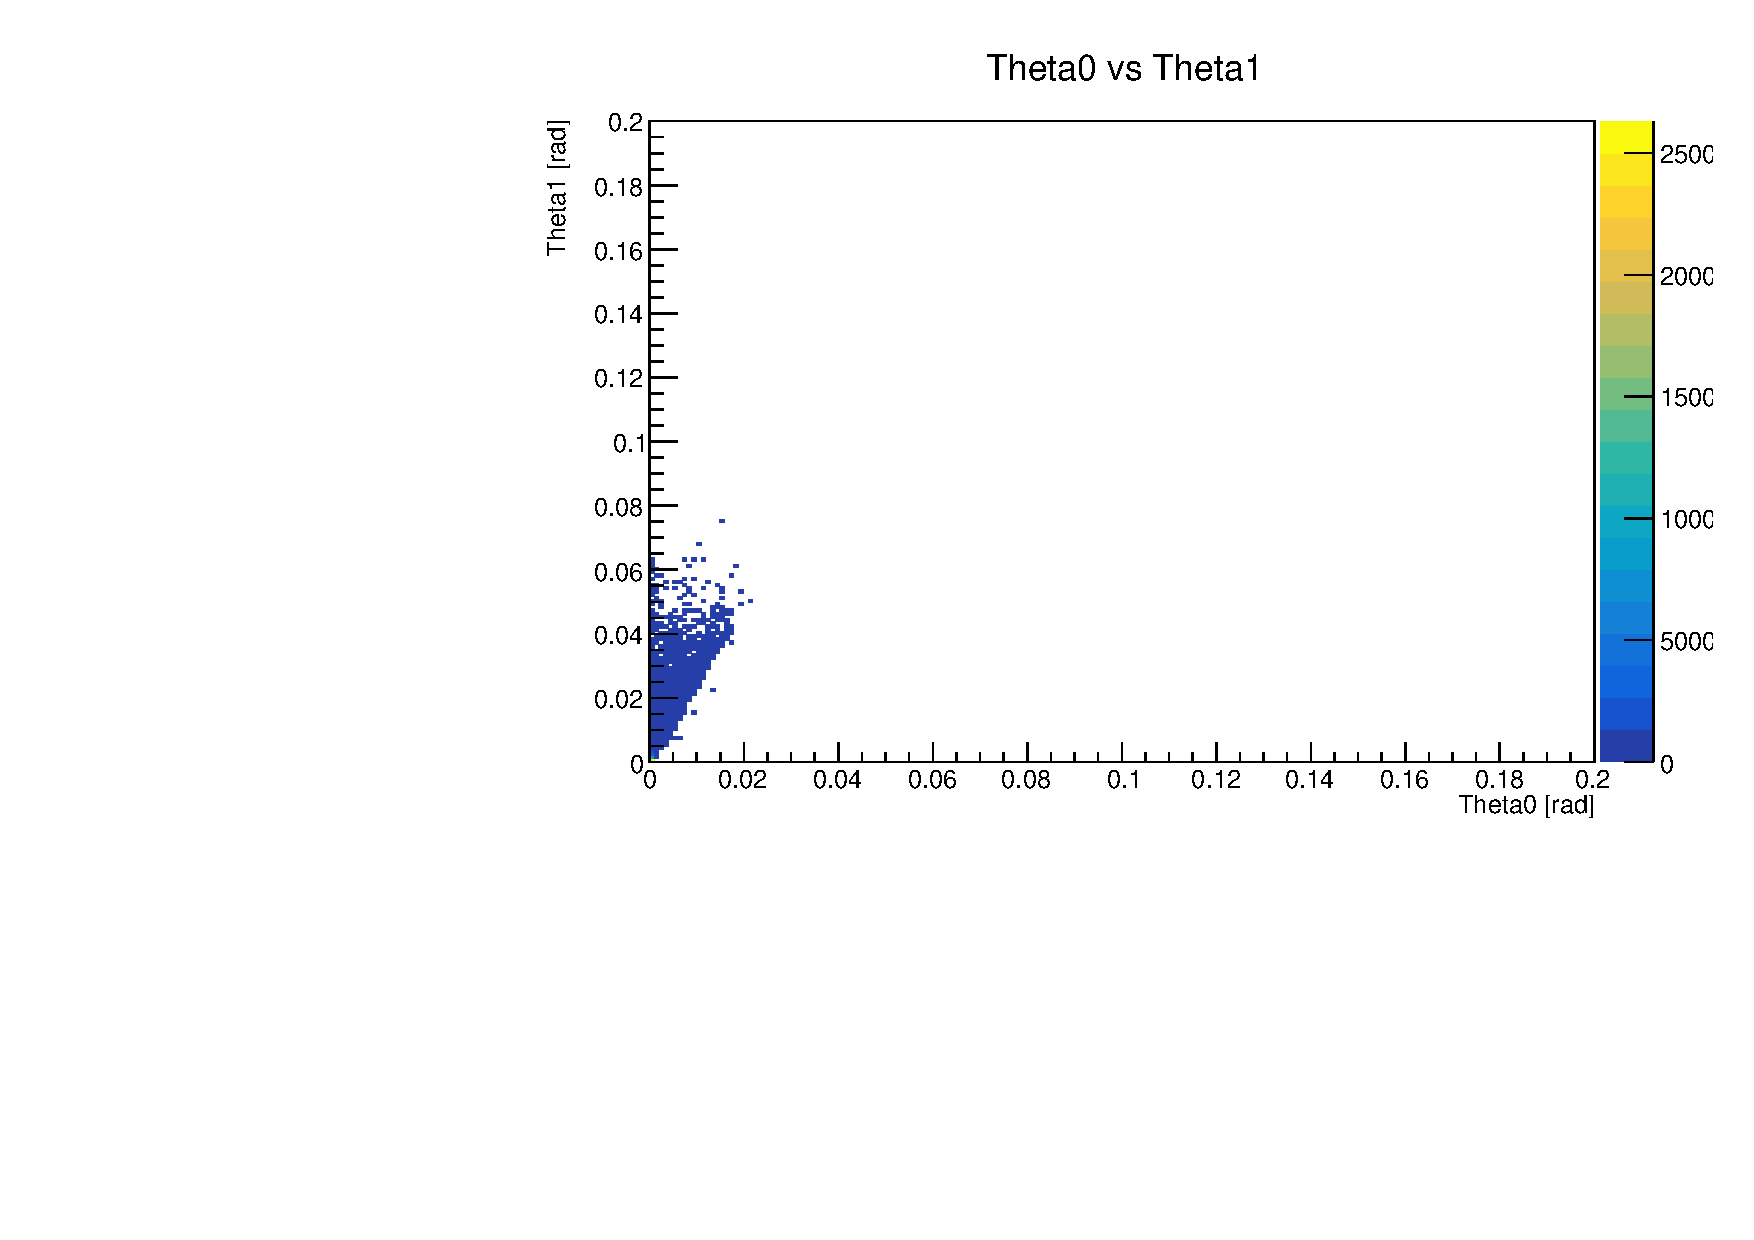
\includegraphics[width=\linewidth]{output/Theta0 vs Theta1.pdf}
	\end{figure}
\end{frame}


% \begin{frame}{Distribution of DeltaRP}
% 	\begin{figure}
% 		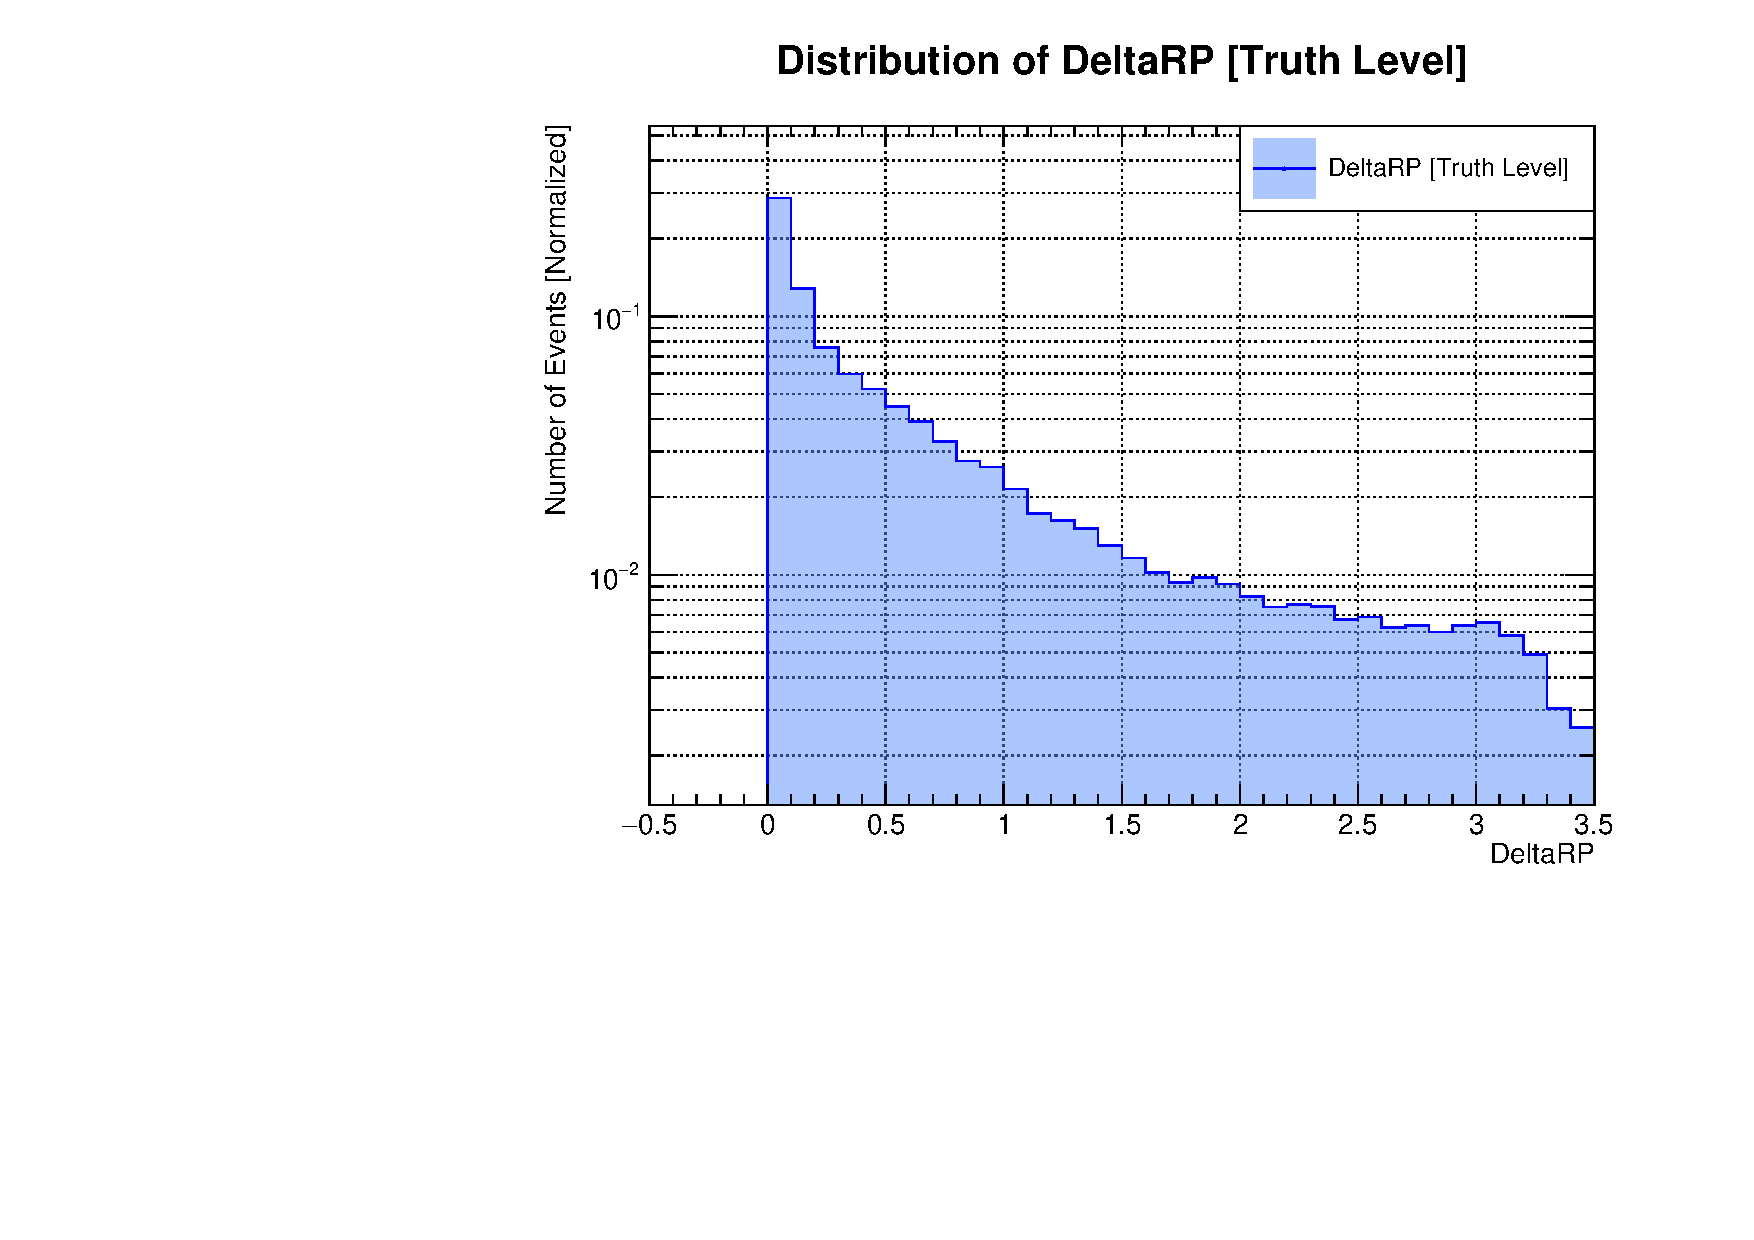
\includegraphics[width=\linewidth]{output/DeltaRP.pdf}
% 	\end{figure}
% \end{frame}

% \begin{frame}{Comments on Position Based Separation}
% 		\begin{itemize}
% 			\item Particle predominantly separated in the y-direction
% 			\begin{itemize}
% 				\item This deflection is caused by the magnetic field.
% 				\item The positron deflected upwards, electron downwards.
% 				\item Giving the asymmetry in DeltaY
% 				\item DeltaX looks symmetric but separation here is much lower
% 				\item Thus, DeltaY can be approximated to DeltaR
% 			\end{itemize}
% 			\item DeltaR1 is more spread out than DeltaR0 due to increased deflection while traversing the magnetic field.
% 			\item Nothing post 0.02 in Theta0 is reconstructed at Theta1 [Verify at event level]
% 		\end{itemize}
% \end{frame}





